\section{Reading the bound}
\label{sec:reading}

The two bounds are stated in different currencies: the elementary one needs no approximation theory, the sharpened one buys a factor $e$ with the whole band.

\paragraph{The two coefficients.} The elementary bound uses flatness alone. Order-$N$
matrix robustness forces the carrier $h$ of~\eqref{eq:h} to vanish to order $q=2N+2$ at
$\lambda=1$ (Proposition~\ref{prop:flatness}), and with $|h^{(q)}|\le\tauvar^{q}$,
$\tauvar=T/2$, one Taylor--Lagrange step at the endpoint gives the inequality of
Theorem~\ref{thm:elementary}. Its coefficient of $N$ is $4/e\approx1.4715$, with no
threshold in $N$ and no approximation theory. The sharpened bound uses the
whole band instead. The $q$ vanishing derivatives at $\lambda=1$ are $q$ vanishing
moments, into which a polynomial of degree $q-1$ can be inserted; approximating
$e^{-i\mu}$ on the band $|\mu|\le\tauvar$ that way, with a compactly supported smoothing,
makes $h(0)$ exponentially small in $q$ whenever $\tauvar\le\rho q$ with fixed $\rho<1$,
which the endpoint separation~\eqref{eq:h0lower} forbids. Carrying the constants through
gives $T\ge4(N+1)[1-a(\log q/q)^{2/3}]$ for every $a\ge2$ and $N\ge N_0(a)$
(Theorem~\ref{thm:main}), a coefficient approaching $4$. The two bounds have the same
shape, a constant times $(N+1)$: the factor $e$ between $4/e$ and $4$ is what the band
supplies over one Taylor remainder.

\paragraph{Where the sharpened term takes over.} Table~\ref{tab:twolayers} evaluates both
at sample orders: the elementary term is the larger one at $N=5$ and $N=10$ ($10.58$
against $4.7$; $18.11$ against $16.6$), the sharpened expression passes it at $N=12$,
i.e.\ $q=26$ ($22.1$ against $21.1$), and beyond that their ratio tends to $e$. Below
$N_0(a)$ the sharpened term is switched off in~\eqref{eq:allN}, so between $N=12$ and
$N_0$ the proved bound is still the elementary one: the crossover locates the order from
which whole-band information begins to pay, not a point at which the proved coefficient
changes. Both terms grow linearly with the same $(N+1)$ normalization, so the comparison
is one of constants: at least $4(N+1)/e$ at every order, and $(1-o(1))\,4(N+1)$ at
large order.

\paragraph{What the pair rules out.} At every order the cost is bounded below by the
elementary bound, hence by $4(N+1)/e$: no arrangement of free rotations, however many,
makes high-order robustification sublinear. The sharpened bound gives $\cstar(\pi)\ge4$; the equiangular family of~\cite{Low2014} gives $\cstar(\pi)\le2\pi$, so
\begin{equation}
4\;\le\;\cstar(\pi)\;\le\;2\pi ,
\label{eq:window}
\end{equation}
an interval of width $2\pi-4\approx2.28$, whose endpoints differ by the factor $\pi/2$; the numerical costs of
Section~\ref{sec:numerics} follow $T\approx5.26N+2.81$ over $N\le8$, within a factor
$2.0$ of the floor at $N=1$ and $1.4$ at $N=8$, so what remains to be found is a bounded correction rather than a new
regime. And since the model already grants exact, instantaneous, free $X$ rotations in
unlimited number and arbitrary placement, and a target reached exactly at the nominal
error, the intuition that a rich enough fast-control layer makes the uncertain evolution
asymptotically efficient is false here.

\paragraph{Why the idealization makes the bounds conservative.} The model is thin by design and every assumption favors the designer: one common multiplicative error, no time dependence, no decoherence, no leakage, instantaneous and perfect transverse control. Any model closer to a laboratory adds constraints, and adding constraints can only raise the least cost of an order-$N$ robust sequence.

\paragraph{Finite order, incoherent errors, and the orders that matter.} A device does
not get to choose $N$ freely: a longer sequence also spends more time in the presence of
decay, the tension that shapes time-optimal gate design on Rydberg platforms~\cite{Jandura2022}. Writing $\omega$ for the rate at which the uncertain $Z$-phase
accumulates and $\gamma$ for the decay rate, an order-$N$ sequence of cost $T$ pays an
incoherent infidelity of order $\gamma T/\omega$ while its coherent error falls like
$\eps^{N+1}$, and the two balance at
\begin{equation}
N^\ast\;\approx\;\frac{\ln(\omega/\gamma)}{2\ln(1/\eps)},
\label{eq:nstar}
\end{equation}
so the useful order grows only logarithmically as coherence improves. At the parameters of Figure~\ref{fig:phys} the estimate gives $N^\ast\approx3.0$, up to the order-one prefactor of the coherent term; the tabulated sequences place the minimum at $N^\ast=2$.

This is where the
finite-order form of the bounds matters: the relevant orders are small, and there the
operative term of~\eqref{eq:allN} is the elementary one, which supplies the cost side of
the balance at every order and without a threshold --- each order costs at least
$2[(2N+2)!]^{1/(2N+2)}\ge4(N+1)/e$ units of accumulated uncertain phase. The incoherent
floor is thus not a property of a particular composite construction, and the tradeoff
cannot be evaded by inventing better pulses, only by improving $\gamma$, $\eps$, or the
resource model itself. Figure~\ref{fig:phys} evaluates the balance at parameters
representative of current neutral-atom arrays: the optimum is at $N^\ast=2$, and improving
$\gamma/\omega$ by three orders of magnitude moves it only to $4$. The panel uses the
tabulated costs of Table~\ref{tab:num}; replacing them by the rigorous floor of~\eqref{eq:allN} lowers the incoherent term but not the coherent one, so the minimum stays
at small order.

\begin{figure}[t]\centering
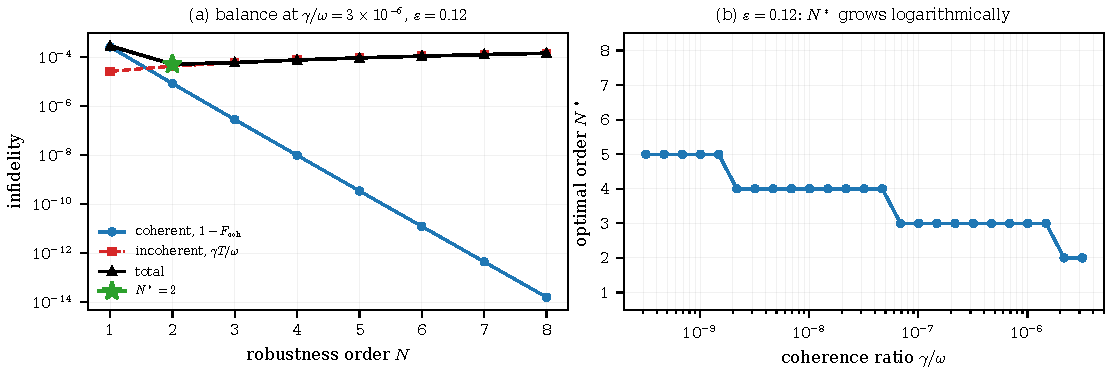
\includegraphics[width=\linewidth]{figphys.pdf}
\caption{The coherent-versus-incoherent balance at parameters representative of current
neutral-atom arrays: interaction strength $V/2\pi\approx500$~MHz at $2\,\mu$m separation~\cite{Evered2023} with Rydberg lifetimes of order $10^2\,\mu$s~\cite{Beterov2009}, i.e.\ a coherence
ratio $\gamma/\omega\approx3\times10^{-6}$, and a systematic variation $\eps=0.12$ of the
interaction. (a) the coherent infidelity $\sin^2(\delta(\eps)/2)$ of the sequences of
Table~\ref{tab:num}, the incoherent infidelity $\gamma T/\omega$ they accumulate, and the sum; the
minimum is at $N^\ast=2$. (b) the same balance over four decades of the coherence ratio: the
optimum moves only to $N^\ast=5$. The sequences plotted are those of Table~\ref{tab:num} with $N\le8$. The coherent term is measured for the tabulated sequences and is therefore an
upper bound on what a better construction of the same order could reach.}
\label{fig:phys}
\end{figure}

\section{Discussion}
\label{sec:discussion}

The bounds are lower bounds on a resource, not a pulse-design prescription. Free and
exact $X$ rotations can rearrange how the systematic $Z$ error accumulates, but when the
common $Z$ scale is turned down to $\lambda=0$ every costly evolution disappears, and the
carrier must connect two separated endpoints while being extremely flat at $\lambda=1$.

\paragraph{What is machine-checked.} The elementary bound is formalized for every order
$N$ and every target $0<\phi\le\pi$ (\path{RobustZ.elementary_bound}, with
\path{elementary_bound_pi} the case $\phi=\pi$), together with the pointwise
comparison $4(N+1)/e<2[(2N+2)!]^{1/(2N+2)}$
(\path{elementary_gt_four_over_e}). The sharpened bound and the combined statement
\path{all_N_bound_end} behind~\eqref{eq:allN} are formalized at $\phi=\pi$: the
target angle enters the whole-band argument only through the endpoint separation
$h(0)\ge2\sin^{2}(\phi/4)$, so the same constants give the general-$\phi$ form, but the
assembled numerical statement in the development is the case $\phi=\pi$
(Section~\ref{sec:formal}). Both explicit constants, including the thresholds, are part
of the checked statements.

\paragraph{Thresholds and numerics.} The thresholds $N_0(a)$ are sufficient conditions
assembled from explicit constants --- a cutoff-derivative constant, an approximation rate
for $e^{-i\mu}$ on the band, and kernel bookkeeping. The exponent $2/3$ in~\eqref{eq:thm-sharp} is the reciprocal of the exponent $3/2$ in that rate: with
$1-\rho=a(\log q/q)^{2/3}$ the exponential gain behaves like $q^{-a^{3/2}}$ against a
polynomial loss, so any fixed $a$ above a bound determined by them
suffices, and the condition $a\ge2$ with the thresholds $5010$ and $46000$ is conservative
bookkeeping rather than a feature of the control problem. The sharpened statement being
vacuous below $N_0$ is therefore not evidence that the coefficient is smaller there;
those orders are covered by the elementary bound.

\paragraph{The exact finite-order question.} It is natural to ask whether the linear
bound can be made exact at finite order, in the form $T\ge4N$ at $\phi=\pi$. The carrier argument uses four properties of $h$:
exponential type $\tauvar=T/2$, a zero of order $q=2N+2$ at $\lambda=1$, a sup bound, and
the endpoint value at $\lambda=0$. Every rescaled carrier has exponential type $1$, $g^{(k)}(0)=0$ for $k<q$, $\lvert g\rvert\le1$ on $\R$ and $\lvert g(-y)\rvert\ge1/2$ at $y=\tauvar$. Let $y_*(q)$ be the least admissible $y$; then $y_*(q)\le\tauvar$, and $T\ge4N$ is exactly $y_*(q)\ge q-2$. Any proof that uses only those four properties proves a lower bound
valid for $y_*(q)$ as well.

That relaxation has been solved numerically, and it does not obey the target. On
commensurable frequency grids, with the sup-norm constraint enforced globally on one
period, certified by a Bernstein correction, and with the moment residuals at machine
precision, explicit exponential sums with $y<q-2$ exist from $q=44$, that is $N=21$,
upward; the smallest witness found has $T=83.44$ against $4N=84$, and the saving grows
with $N$, reaching about $17\%$ at $N=29$ ($T=96$ against $116$). The grid restricts the
admissible class, so such a solution is a witness for the continuum relaxation as well;
the first beating order moves down from $q=46$ to $q=44$ when the grid is refined, and
none was found below it. The conclusion is negative but useful: the finite-order
statement $T\ge4N$ cannot be obtained from the analytic data of the carrier --- band,
flatness, sup bound, endpoint value --- and any proof of it must use the product structure
of~\eqref{eq:sequence}: that $h$ is the trace overlap
$1-\tfrac12\Ree\Tr(U_1^\dagger U_\lambda)$ of an $X$--$Z$ product with $\theta_j\ge0$ and
$\sum_j\theta_j=T$, so that its frequencies are the half-sums
$\tfrac12\sum_js_j\theta_j$ with $s_j\in\{\pm1\}$, and its endpoint value is tied to the
free rotations through $h(0)=1-\cos(\phi/2)\cos(A/2)$ of~\eqref{eq:h0exact}. None of that
structure survives the relaxation, whose extremals are edge-dominated packets alternating
in parity with $q$.

\paragraph{The constant is not proved optimal.} The whole-band argument proves the left
half of~\eqref{eq:window} and leaves a genuine gap: equality would require a matching
upper-bound construction in the precise free-$X$ model.

\section{Conclusion}
\label{sec:conclusion}

We have established explicit lower bounds on the $Z$-evolution cost of high-order robust
composite $Z$ rotations, in a model where the imperfect $Z$ evolution is the only costly
operation and exact $X$ rotations are free. For every order $N\ge1$ and every target
$0<\phi\le\pi$ the elementary bound gives
$T\ge2[2(2N+2)!\sin^{2}(\phi/4)]^{1/(2N+2)}$, a coefficient $4/e\approx1.4715$. Using the whole frequency band of the carrier as well
gives, at $\phi=\pi$, $T\ge4(N+1)[1-a(\log q/q)^{2/3}]$ for every $a\ge2$ and every
$N\ge N_0(a)$, with the explicit threshold $N\ge5010$ at $a=2.3$, so that the coefficient
approaches $4$. Taking the
larger of the two at each order yields a single bound valid at every order
(Corollary~\ref{cor:allN}), of which the familiar asymptotic statement
$\liminf_{N\to\infty}T_{\min}(N,\phi)/N\ge4$ is a corollary. Both constants, and the
thresholds that come with them, are machine-checked in Lean~4 with Mathlib.

What remains open is a sharper finite-order statement. The numerical constructions of
Section~\ref{sec:numerics} are admissible sequences whose nominal identity and order $N$
were re-verified independently, and they show that the equiangular value
$2\pi$ is not optimal; being upper bounds from a local search, they determine no value of $\cstar(\pi)$. In the other direction, the
relaxation discussed above shows that the exact statement $T\ge4N$ cannot be reached from
the analytic data of the carrier, since certified band-limited constructions with $T<4N$
exist from $N=21$ on. Closing the gap between $4/e$ and $4$, or proving a bound exact at
finite order, therefore requires an argument that uses the product structure of~\eqref{eq:sequence} rather than the carrier alone; at the orders a device actually uses,
the elementary bound is the one that applies.
